\chapter{Requirement Analysis}

\section{Overview}
In this chapter, there will be a discussion about the requirements of the project. Requirement analysis is the process of identifying, analyzing, and documenting the needs and expectations of the stakeholders for a software system. It is the first and most crucial step in the software development life cycle, and it involves understanding the user’s requirements and the system’s objectives. In this project, we have used VS code for building the online system. Here we use different types of language such as; HTML, CSS, and JavaScript. We also use SQL for a database where we store all information such as teacher information, student information, questions, tasks etc.

\section{User Requirement}
Any system, including web-based systems, must take the needs of its users into consideration when being designed and developed. The needs, expectations, and preferences of the system's users must be determined and given top priority while developing a web-based student evaluation system. A web-based student evaluation system is often used primarily by students, teachers, and administrators. It is crucial to comprehend their needs in order to make sure the system fits them and offers a positive user experience. Here are some important things to remember for each user group.
\begin{figure}[H]
    \centering
    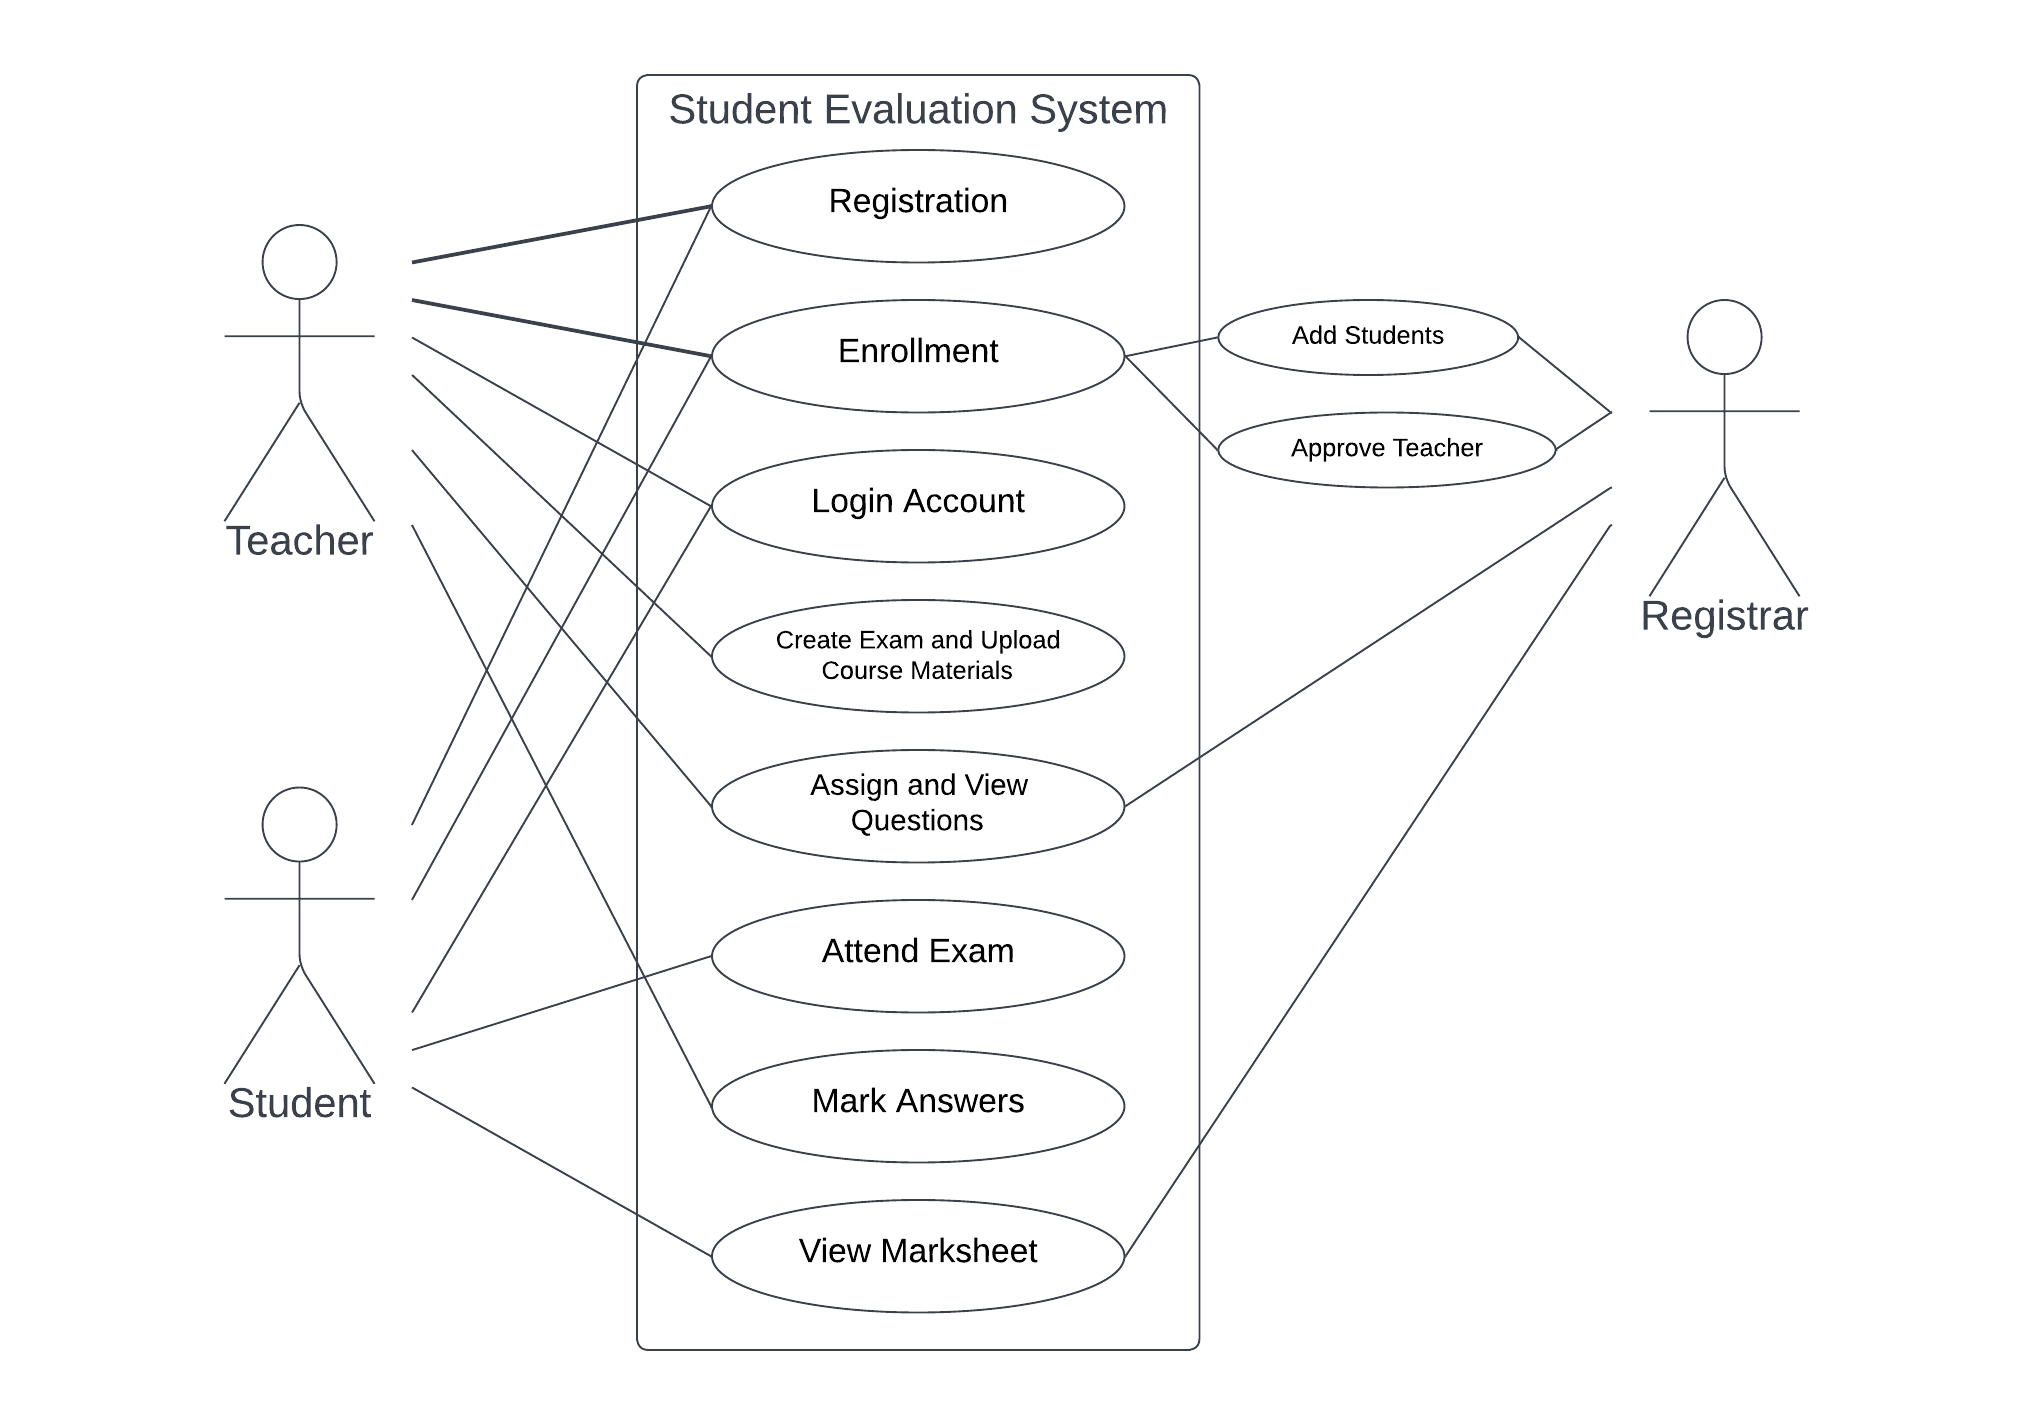
\includegraphics[scale=.2]{img/caseuml.png}
    \caption{Use Case Diagram}
    \label{fig:uml}
\end{figure}
A non-functional diagram provides an overview of the different aspects and characteristics of a system or process without detailing its internal workings. When it comes to online student evaluation, a non-functional diagram helps illustrate the non-functional requirements or qualities that the system should possess. The following figure of a non-functional diagram for an online student evaluation system illustrates the process to get registered as a user whether the user is a teacher or a student.\\

The functional diagram provides an overview of the system's major functions and their interdependencies. It helps stakeholders and system designers understand the flow of information and actions within the system, guiding the development and implementation process. 
Additionally, the functional diagram can serve as a basis for further decomposition into more detailed functional specifications for each component, ensuring a comprehensive and well-structured system design. 
\begin{figure}[H]
    \centering
    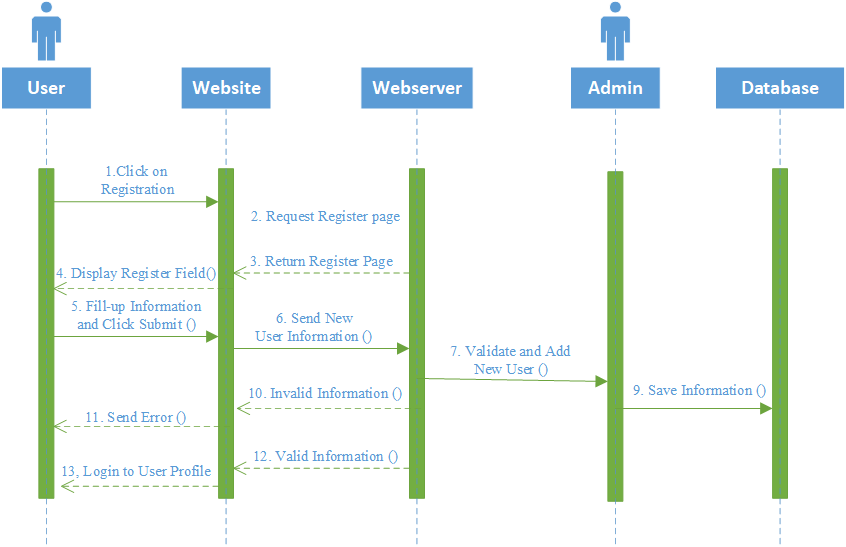
\includegraphics[scale=.7]{img/User.png}
    \caption{User Registration}
    \label{fig:uml1}
\end{figure}
In the case of an online student evaluation system, a functional diagram outlines the key functionalities and their relationships. The following figures show how a user can log in to the system and after being logged in what types of information the user will get.

\begin{figure}[H]
    \centering
    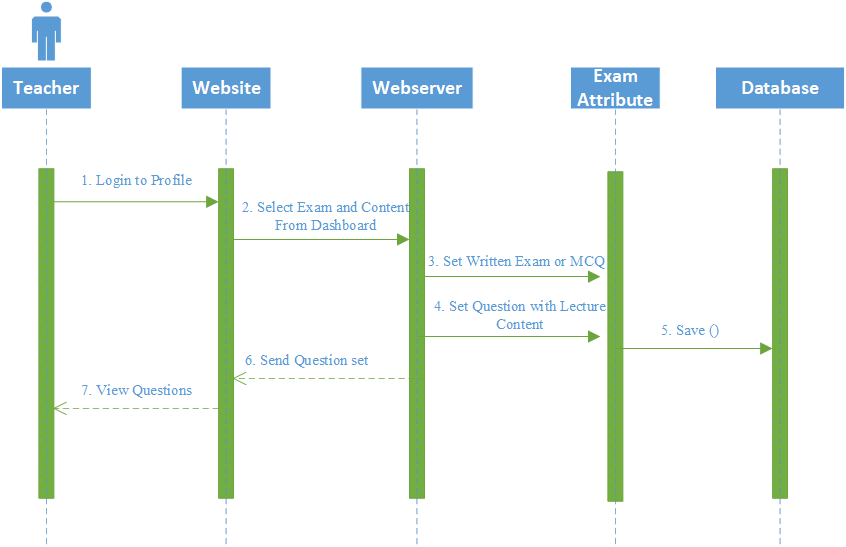
\includegraphics[scale=.7]{img/teacheruml.png}
    \caption{Teacher Set Question}
    \label{fig:uml2}
\end{figure}
From the above figure, we can see that a teacher will be able to create an exam and also there will be options to make both questions MCQ or written. The teacher will also be able to edit the questions if it is needed.
\begin{figure}[H]
    \centering
    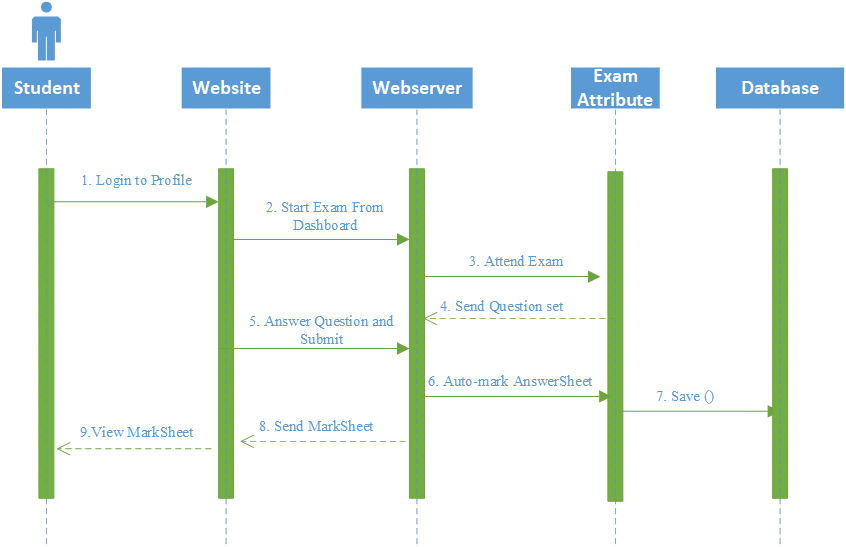
\includegraphics[scale=.7]{img/studentuml.png}
    \caption{Student Exam Attend}
    \label{fig:uml3}
\end{figure}
The above figure clearly shows that a student will be able to view the questions, attend the exams and submit the answer scripts. They will also be able to view the mark sheet of a particular exam from the website. 

\section{Software Requirement} 
This section explained software requirements, their importance, and their role in the development process. Software requirements serve as a foundation for designing, developing, and delivering successful software systems that meet the needs and expectations of users and stakeholders.

\subsection{VS code}
Visual Studio Code (VS Code) is a lightweight, cross-platform source code editor developed by Microsoft. It is free and open-source and supports a wide range of programming languages, making it a popular choice for developers worldwide. VS Code supports debugging for various programming languages, allowing developers to identify and fix bugs in their code. It has a vast library of extensions that provide additional functionality to the editor, making it more efficient and productive. VS Code comes with an integrated terminal that allows developers to run commands, scripts, and programs within the editor itself. The platform has built-in Git integration, enabling developers to manage source code repositories directly from the editor.
\subsection{Browser} 
Spider Browser is a modern and feature-rich web browser designed to provide users with a fast, secure, and customizable browsing experience. It offers a range of functionalities and tools that enhance productivity, privacy, and convenience while navigating the web.The customization options allow users to adapt the browser's appearance and functionality to their preferences, creating a personalized browsing experience. Spider Browser's optimized performance ensures fast and efficient browsing, enabling users to access web content quickly and smoothly.


\section{Language Requirement}
The section provides an overview of programming language requirements, their significance in software development, and their role in determining the choice of programming languages for different projects. Programming language requirements help define the specific programming languages that need to be used to develop software systems based on project needs and constraints.

\subsection{HTML}y
HTML (Hypertext Markup Language) is a markup language used to create and design web pages. It is the foundation of all web development and is used to structure and display content on the internet. HTML provides a set of elements or tags that define the structure and appearance of web pages. HTML is constantly evolving, with new versions introducing new features and improvements to existing ones. The latest version of HTML is HTML5, which includes new elements and features for multimedia, graphics, and interactive content.

\subsection{CSS} 
CSS (Cascading Style Sheets) is a stylesheet language used to describe the presentation and styling of HTML documents. It is used to control the layout, design, and visual appearance of web pages. CSS uses selectors to target specific elements in HTML and apply styles to them. Selectors can be based on element type, class, ID, attribute, and more. It provides a range of layout options, including grid, flexbox, and float. These layout options allow developers to create complex and responsive layouts for web pages. 

\subsection{JavaScript}
JavaScript (JS) is a high-level, dynamic, and interpreted programming language that is widely used to add interactivity and functionality to web pages. It is a client-side scripting language, meaning that it runs on the user's web browser rather than on a server. Javascript allows us to mark the mcq using local browser cookies of the examinee. It allows developers to write asynchronous code using callbacks, promises, and async/await, which enables the development of complex and efficient web applications.

\subsection{SQL} 
SQLite is a lightweight, open-source, and self-contained relational database management system (RDBMS) that is widely used in various software applications, including web and mobile apps. It is a serverless database, meaning that it does not require a separate server process to function and can be embedded directly into an application. SQLite is cross-platform and can be used on various operating systems, including Windows, macOS, Linux, and mobile operating systems like Android and iOS. 

\subsection{Django}
Django is a high-level, open-source Python web framework that is designed to help developers build complex, scalable, and maintainable web applications quickly and easily. It follows the Model-View-Controller (MVC) architectural pattern and emphasizes the "Don't Repeat Yourself" (DRY) principle, which aims to reduce code duplication and increase efficiency.
Django includes a powerful FORM that allows developers to work with databases using Python objects, rather than directly writing SQL code. It includes a powerful URL routing system that allows developers to map URLs to views, which are Python functions that handle HTTP requests. It also includes built-in security features, such as protection against SQL injection attacks and cross-site scripting (XSS) attacks.




